\documentclass[11pt]{article}
\parindent 0px 
\usepackage{fullpage}
\usepackage{graphicx}
\usepackage{amsmath}

\begin{document}

\section{PINN Method}

\subsection{Neural Networks}
The Artificial Neural Network (ANN) is a computational approach to modeling the biological neural 
network's structure and functionality. ANNs are made up of connected units known as neurons,
and these are organized in layers: there is an input layer, one or several hidden layers, and an output layer. 
A weight is assigned to each link, defining the strength of the information transmission across it.

In feedforward networks, information travels through successive layers from input to output,
passing first through hidden layers. In each node, information enters and is processed,
undergoing weighted addition and then nonlinear transformation with the use of an activation function. 
The training process involves modifying the network's parameters according to a loss function using algorithms 
for gradient descent such as backpropagation.

Neural networks are universal function approximators, meaning that, given enough training samples, 
they can approximate any continuous function. 
As a result of their capacity to discover intricate non-linear links between inputs and outputs, 
neural networks have found numerous applications in a variety of fields like image processing, text recognition, 
scientific computation, and the resolution of differential equations.
In the context of Physics-Informed Neural Networks (PINNs), neural networks are employed to 
approximate the solution of a differential 
equation while simultaneously satisfying the governing physical laws through additional c
onstraints incorporated into the loss function.[1]


Mathematically, a feed-forward neural network can be understood as a composition of several functions. Each layer transforms the output of the previous layer until the final output is produced. If the network has (L) layers, then the approximation can be written as

$$F_L \circ F_{L-1} \circ \cdots \circ F_1(t,x)$$


where each $(F_i)$ represents the transformation performed by the $(i)-th$ layer. This layered structure allows the network to build increasingly complex representations of the solution.


\begin{figure}[h]
    \centering
    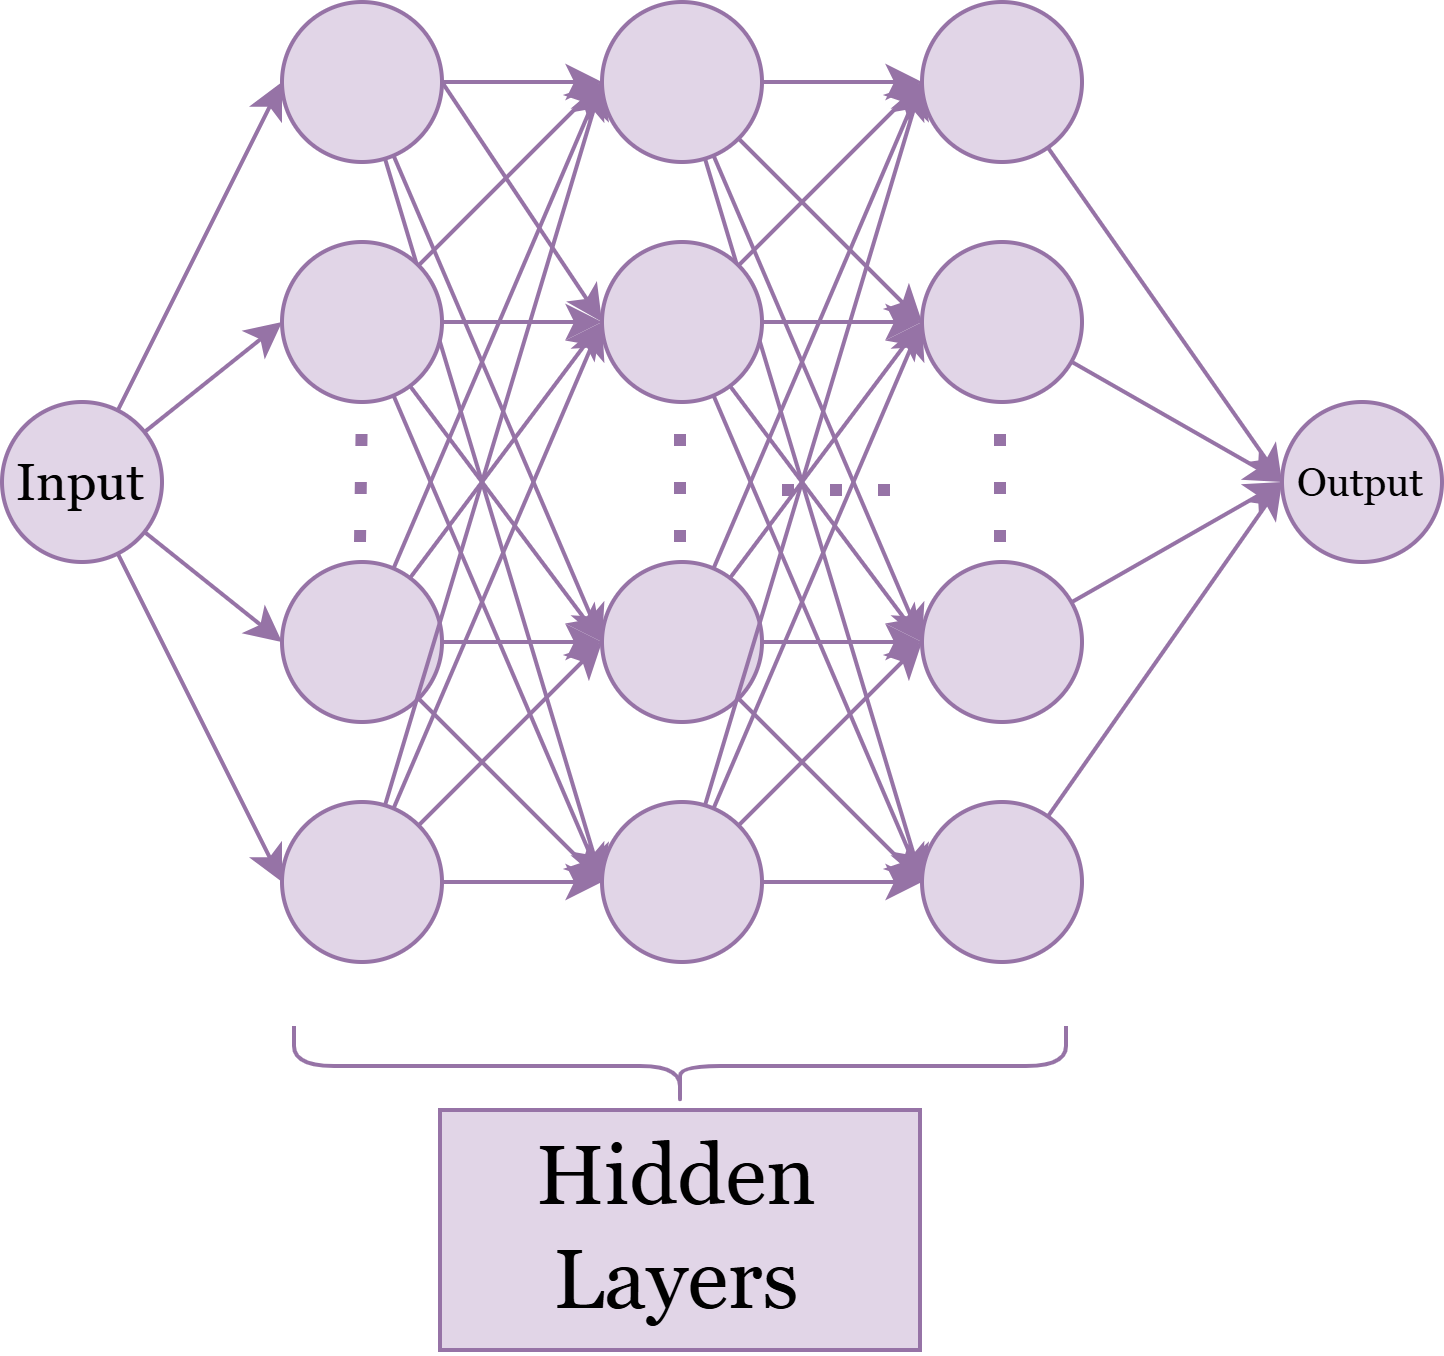
\includegraphics[width=.4\textwidth]{Neural_Network.png}
    \caption{Nerual Network}
    \label{fig:nn}
\end{figure}

\vspace{3in}

\subsection{PINNs}
The conventional neural network is trained with the help of data only. If we provide some data samples to 
the network, the network tries to minimize the error between the predicted output values and the observed
 values. Though this methodology has produced very good results in many different scenarios, it needs plenty 
 of data and does not ensure that the solution that is predicted by the model complies with the physical laws.

On the other hand, Physics-Informed Neural Networks (PINNs) combine the concept of a neural network with the 
physical laws governing the system. Unlike a standard neural network, which is trained using data only, 
a PINN is constrained by physical laws represented by a Partial Differential Equation (PDE). 
Here, the neural network is responsible for approximating the unknown solution $(u(t,x))$, whereas automatic
differentiation is used to calculate the necessary derivatives in the PDE.
For a general PDE of the form

\begin{equation}
u_t + \mathcal{N}[u] = 0
\end{equation}



the neural network predicts the solution $(u(t,x))$. Using automatic differentiation, 
the derivatives $(u_t), (u_x), (u_{xx})$, and higher-order terms can be computed exactly with respect to the network inputs. 
These derivatives are then substituted into the governing equation to form a residual function

\begin{equation}
f(t,x) = u_t + \mathcal{N}[u].
\end{equation}

In case the neural network adheres exactly to the physical law, then the residual 
(f(t,x)) is supposed to take the value of zero throughout the whole domain. 
Hence, there will be two components in the training process of a PINN. 
One is related to the data error while the other component relates to physics, 
which serves as an additional constraint.

A PINN may therefore be regarded as a neural network that makes use of both 
observation data as well as the principles of physics. The incorporation of 
such physical knowledge provides additional information for the network, 
which works as a regularization technique.



\begin{figure}[h]
    \centering
    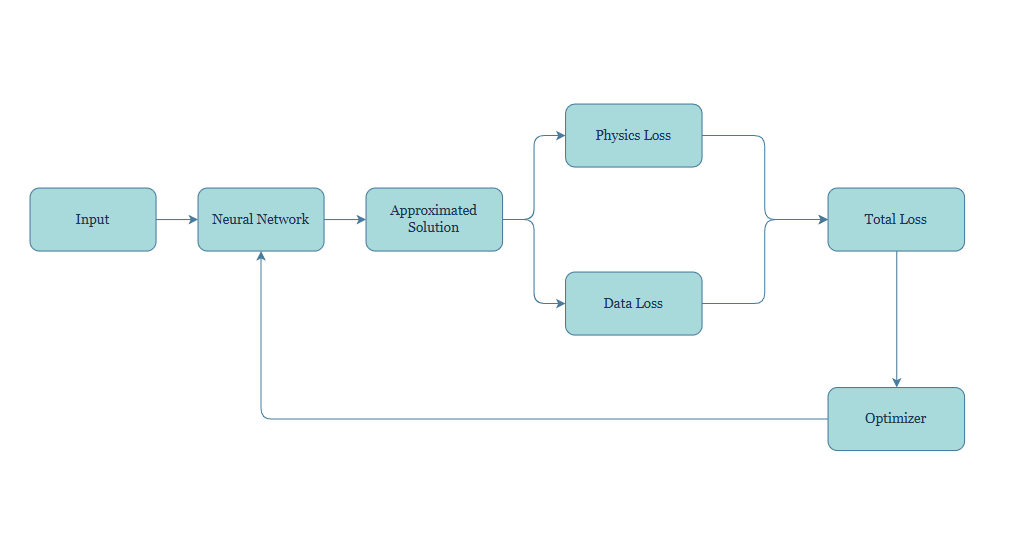
\includegraphics[width=1\textwidth]{pinn_framework.png}
    \caption{PINN Framework} 
    \label{fig:pinns}
\end{figure}


\subsection{Implenetation}

The architecture of a Physics-Informed Neural Network is typically implemented based on a 
fully connected feed-forward neural network, though in many cases they try many other architecture for NN. 
In this structure, the input layer receives the independent variables of 
the problem. For a time-dependent one-dimensional PDE, these inputs are 
usually the spatial coordinate $(x)$ and the time variable $(t)$. 
Therefore, each input point can be shown as $(x,t)$. The role of the 
neural network is mapping this input point to the corresponding approximation of the unknown solution. 
In other words, the network represents the function

\begin{equation}
u_\theta(x,t) \approx u(x,t)
\end{equation}
where $(\theta)$ denotes all trainable parameters of the neural network, including weights and biases[lulu]

In the traditional neural network, the output of the architecture is checked only with available data. However, the output from the architecture in a PINN is
further taken to the physics-based part of the algorithm. 
This means that after the network predicts $u_\theta(x,t)$, automatic differentiation is applied to 
compute the derivatives required in the PDE, such as


\begin{equation}
\frac{\partial u_\theta}{\partial t},
\frac{\partial u_\theta}{\partial x},
\frac{\partial^2 u_\theta}{\partial x^2}.
\end{equation}

[raissi2019.pdf]



To evaluate how well the governing equation is satisfied, 
PINNs introduce a set of collocation points inside the computational domain. 
These points are sampled throughout the domain and are not necessarily 
associated with any observed data. Let the collocation points be denoted by

${(x_f^i,t_f^i)}_{i=1}^{N_f}$

where $(N_f)$ represents the number of collocation points. 
At each of these points, the residual $(f_\theta(x,t))$ is evaluated. If the residual is large at a particular location, it indicates that the neural network 
prediction violates the governing 
equation at that point. Consequently, the network parameters are 
adjusted to reduce this error. One important advantage of this approach is 
that PINNs are mesh-free methods and therefore do not require the computational mesh used by traditional 
numerical techniques such as the Finite Element Method or Finite Difference Method. [raissi2019] [Cuomo2022]


The learning process of a PINN is controlled through a loss function that combines 
information from both the available data and the governing physics. 
In the most general case, the total loss function consists of four components:
$$
\mathcal{L_{\textsl{data}}}
+
\mathcal{L_{\textsl{physics}}}
+
\mathcal{L_{\textsl{boundary}}}
+
\mathcal{L_{\textsl{initial}}}
$$

The data loss measures the difference between the neural network 
predictions and the available observations. The physics loss 
evaluates how well the governing differential equation is 
satisfied at the collocation points. The boundary loss enforces 
the prescribed boundary conditions, while the initial loss 
ensures that the initial conditions are satisfied. Together, 
these terms guide the network toward a physically meaningful solution.[raissi2019]
More specifically, the physics loss is often defined as the mean squared value of 
the PDE residual evaluated at all collocation points:
\begin{equation}
frac{1}{N_f}
\sum_{i=1}^{N_f}
\left|
f_\theta(x_f^i,t_f^i)
\right|^2
\end{equation}


Minimizing this term forces the neural network to satisfy the 
governing equation throughout the computational domain. Similarly, 
if observational data are available, the data loss can be written as


\begin{equation}
\frac{1}{N_u}
\sum_{i=1}^{N_u}
\left|
u_\theta(x_u^i,t_u^i)-u^i
\right|^2,
\end{equation}

where $(u^i)$ denotes the observed value of the solution at the point $((x_u^i,t_u^i))$. [raissi2019]


After the total loss function is constructed, an optimization algorithm such 
as Adam or L-BFGS is used to update the trainable parameters $(\theta)$. 
During each training iteration, the gradients of the loss function with 
respect to the network parameters are computed using backpropagation. 
The optimization process continues until the total loss reaches a sufficiently 
small value, indicating that the neural network simultaneously fits the available 
data and satisfies the governing physical laws. [Lu2021]



\subsection{The Schrödinger Equation and Physics-Informed Neural Networks}

The Schrödinger equation is the fundamental equation of quantum mechanics and 
describes the evolution of a quantum system through its wave function. In its 
time-dependent form, the equation is written as

\begin{equation}
i\hbar \frac{\partial \psi}{\partial t}
=
\hat{H}\psi,
\end{equation}

where $\psi(x,t)$ denotes the wave function, $\hbar$ is the reduced 
Planck constant, and $\hat{H}$ is the Hamiltonian operator. 
The solution of the Schrödinger equation contains complete 
information about the physical system and can be used to 
determine quantities such as probability distributions and energy levels.

The Schrödinger equation plays a central role in many 
scientific fields, including quantum mechanics, 
quantum chemistry, atomic physics, 
condensed matter physics, and quantum computing. 
Because analytical solutions are available only for a 
limited number of simple systems, numerical methods are 
often required to approximate its solutions.

In recent years, Physics-Informed Neural Networks (PINNs) 
have emerged as a promising alternative to traditional numerical 
approaches. By embedding the governing differential 
equation directly into the loss function, PINNs can learn 
solutions that satisfy both observational data and the 
underlying physical laws. This capability makes PINNs particularly
attractive for solving Schrödinger-type equations, where accurate 
approximations of wave functions are required. [wang2021.pdf]

\subsection{Problem Statement}

In this project, we consider the one-dimensional time-dependent 
Schrödinger equation with a harmonic potential

\begin{equation}
i\frac{\partial \psi}{\partial t}
=
-\frac{1}{2}\frac{\partial^2 \psi}{\partial x^2}
+
\frac{1}{2}x^2\psi,
\end{equation}

where $\psi(x,t)$ denotes the complex-valued wave function. The term

\begin{equation}
-\frac{1}{2}\frac{\partial^2 \psi}{\partial x^2}
\end{equation}

represents the kinetic energy contribution, while

\begin{equation}
\frac{1}{2}x^2\psi
\end{equation}

corresponds to the harmonic oscillator potential. 
This equation is one of the most important models in 
quantum mechanics and is frequently used as a benchmark 
problem for numerical and machine learning methods.

To solve this problem using PINNs, the neural 
network receives the spatial coordinate 
$x$ and time $t$ as inputs and approximates 
the wave function $\psi(x,t)$. Automatic d
ifferentiation is then employed to compute 
the derivatives required by the governing equation, 
and the residual of the Schrödinger equation is 
incorporated into the loss function. The network 
parameters are optimized such that the predicted 
solution satisfies both the differential equation 
and the prescribed initial and boundary conditions.
\subsection{Initial and Boundary Conditions}
To obtain a unique solution of the Schrödinger equation, 
appropriate initial and boundary conditions must be specified.
In this work, the spatial domain is defined as

\begin{equation}
    x \in [-5,5]
\end{equation}


while the temporal domain is chosen as

\begin{equation}
    t \in [0,1]
\end{equation}
The initial condition is selected as a Gaussian wave packet,

\begin{equation}
    \psi(x,0)=e^{-x^2}
\end{equation}

which is a commonly used initial state in quantum mechanics 
due to its smoothness and localized nature. Since the wave 
function is represented in terms of its real and imaginary 
components,

\begin{equation}
    \psi(x,t)=u(x,t)+iv(x,t)
\end{equation}

the initial condition can be written as

\begin{equation}
    u(x,0)=e^{-x^2}
\end{equation}


\begin{equation}
    v(x,0)=0
\end{equation}

These conditions are enforced during training through the initial-condition 
loss term, which penalizes discrepancies between the 
neural network predictions and the prescribed initial values.

Furthermore, homogeneous Dirichlet boundary conditions are 
imposed at the boundaries of the spatial domain. 
Specifically,

\begin{equation}
    u(-5,t)=u(5,t)=0
\end{equation}

and

\begin{equation}
    v(-5,t)=v(5,t)=0
\end{equation}


These boundary conditions ensure that the wave function 
remains negligible at the edges of the computational domain, 
which is consistent with the localized nature of the 
Gaussian initial state.

Within the PINN framework, 
both the initial and boundary conditions are 
incorporated directly into the loss function. 
During training, the neural network is required not 
only to satisfy the governing Schrödinger equation but 
also to reproduce the prescribed initial and boundary 
conditions. This enables the network to learn a physically 
consistent approximation of the wave function throughout 
the spatio-temporal domain.



\subsection{PINN Formulation for the Schrödinger Equation}

\subsection{PINN Formulation for the Schrödinger Equation}

To solve the time-dependent Schrödinger equation using Physics-Informed Neural Networks (PINNs), the complex-valued wave function is first decomposed into its real and imaginary components. Thus, the solution is represented as

\begin{equation}
\psi(x,t)=u(x,t)+i\,v(x,t)
\end{equation}

where $u(x,t)$ and $v(x,t)$ denote the real and imaginary parts of the wave function, respectively.

In the PINN framework, a fully connected neural network is employed to approximate these two functions simultaneously. The inputs of the network are the spatial coordinate $x$ and the time variable $t$, while the outputs correspond to the approximations $u_\theta(x,t)$ and $v_\theta(x,t)$, where $\theta$ denotes the trainable parameters of the neural network.

The governing equation considered in this work is

\begin{equation}
i\frac{\partial \psi}{\partial t}
=
-\frac{1}{2}\frac{\partial^2\psi}{\partial x^2}
+
\frac{1}{2}x^2\psi
\label{eq:schrodinger}
\end{equation}

Substituting

\begin{equation}
\psi=u+i\,v
\end{equation}

into the Schrödinger equation and separating the real and imaginary parts yields the coupled system

\begin{equation}
u_t
=
-\frac{1}{2}v_{xx}
+
V(x)v
\end{equation}

\begin{equation}
v_t
=
\frac{1}{2}u_{xx}
-
V(x)u
\end{equation}

where

\begin{equation}
V(x)=\frac{1}{2}x^2
\end{equation}

is the harmonic potential.

Using automatic differentiation, the neural network computes the required derivatives $u_t$, $v_t$, $u_{xx}$, and $v_{xx}$. These derivatives are then used to construct the physics residuals

\begin{equation}
f_u
=
u_t
+
\frac{1}{2}v_{xx}
-
V(x)v
\end{equation}

\begin{equation}
f_v
=
v_t
-
\frac{1}{2}u_{xx}
+
V(x)u
\end{equation}

If the neural network exactly satisfies the Schrödinger equation, both residual functions vanish throughout the computational domain. Therefore, the objective of the PINN is to minimize these residuals while simultaneously satisfying the prescribed initial and boundary conditions.

To enforce the governing equation, a set of collocation points is sampled inside the spatio-temporal domain. At these points, the residuals $f_u$ and $f_v$ are evaluated and incorporated into the loss function. The resulting physics loss is given by

\begin{equation}
\mathcal{L}_{\mathrm{PDE}}
=
\frac{1}{N_f}
\sum_{i=1}^{N_f}
\left(
|f_u(x_i,t_i)|^2
+
|f_v(x_i,t_i)|^2
\right)
\end{equation}

where $N_f$ denotes the number of collocation points.

The total loss function combines the physics loss with the losses associated with the initial conditions, boundary conditions, and available reference data. Therefore,

\begin{equation}
\mathcal{L}
=
\lambda_{\mathrm{PDE}}\mathcal{L}_{\mathrm{PDE}}
+
\lambda_{\mathrm{IC}}\mathcal{L}_{\mathrm{IC}}
+
\lambda_{\mathrm{BC}}\mathcal{L}_{\mathrm{BC}}
+
\lambda_{\mathrm{Data}}\mathcal{L}_{\mathrm{Data}}
\end{equation}

where the coefficients $\lambda_{\mathrm{PDE}}$, $\lambda_{\mathrm{IC}}$, $\lambda_{\mathrm{BC}}$, and $\lambda_{\mathrm{Data}}$ control the contribution of each component during training.
\subsection{Experimetal Setup}

The Physics-Informed Neural Network used in this work is implemented as a fully connected feed-forward neural network. The input layer receives the spatial coordinate $x$ and the time variable $t$, while the output layer predicts the real and imaginary components of the wave function, $u_\theta(x,t)$ and $v_\theta(x,t)$. Consequently, the network has two input neurons and two output neurons.

To approximate the solution of the Schrödinger equation, the network consists of four hidden layers with 64 neurons in each layer. The hyperbolic tangent ($\tanh$) activation function is employed throughout the hidden layers. This activation function is commonly used in PINN applications because it is smooth, differentiable, and well suited for automatic differentiation. The network weights are initialized using the Glorot normal initialization method, which helps stabilize the training process and improves convergence.

During training, collocation points are sampled throughout the computational domain to enforce the governing differential equation. Additional points are selected on the initial surface and domain boundaries to impose the prescribed initial and boundary conditions. Furthermore, reference solution data are incorporated into the training process to improve the accuracy of the learned solution.

The training procedure begins with a forward pass through the neural network. Given an input pair $(x,t)$, the network predicts the corresponding values of $u_\theta(x,t)$ and $v_\theta(x,t)$. Automatic differentiation is then used to compute the required derivatives appearing in the Schrödinger equation, including $u_t$, $v_t$, $u_{xx}$, and $v_{xx}$. These derivatives are subsequently used to evaluate the PDE residuals and the corresponding loss terms.

The total loss function is obtained by combining the physics loss, initial-condition loss, boundary-condition loss, and data loss. Backpropagation is then employed to compute the gradients of the loss function with respect to the trainable parameters of the network. These gradients are used to iteratively update the weights and biases until the network converges to a satisfactory solution.

To optimize the network parameters, a two-stage training strategy is adopted. In the first stage, the Adam optimizer is used to rapidly explore the parameter space and obtain a reasonable approximation of the solution. Adam is particularly effective during the early stages of training because of its adaptive learning-rate mechanism. In the second stage, the L-BFGS optimizer is employed to further refine the solution and improve convergence. This hybrid optimization strategy is widely used in PINN applications because it combines the robustness of Adam with the high-accuracy convergence properties of L-BFGS.

After training is completed, the resulting neural network provides an approximation of the wave function throughout the entire spatio-temporal domain. The accuracy of the learned solution is assessed by comparing the PINN predictions with the reference numerical solution and evaluating the relative $L_2$ error.

\begin{figure}[h]
    \centering
    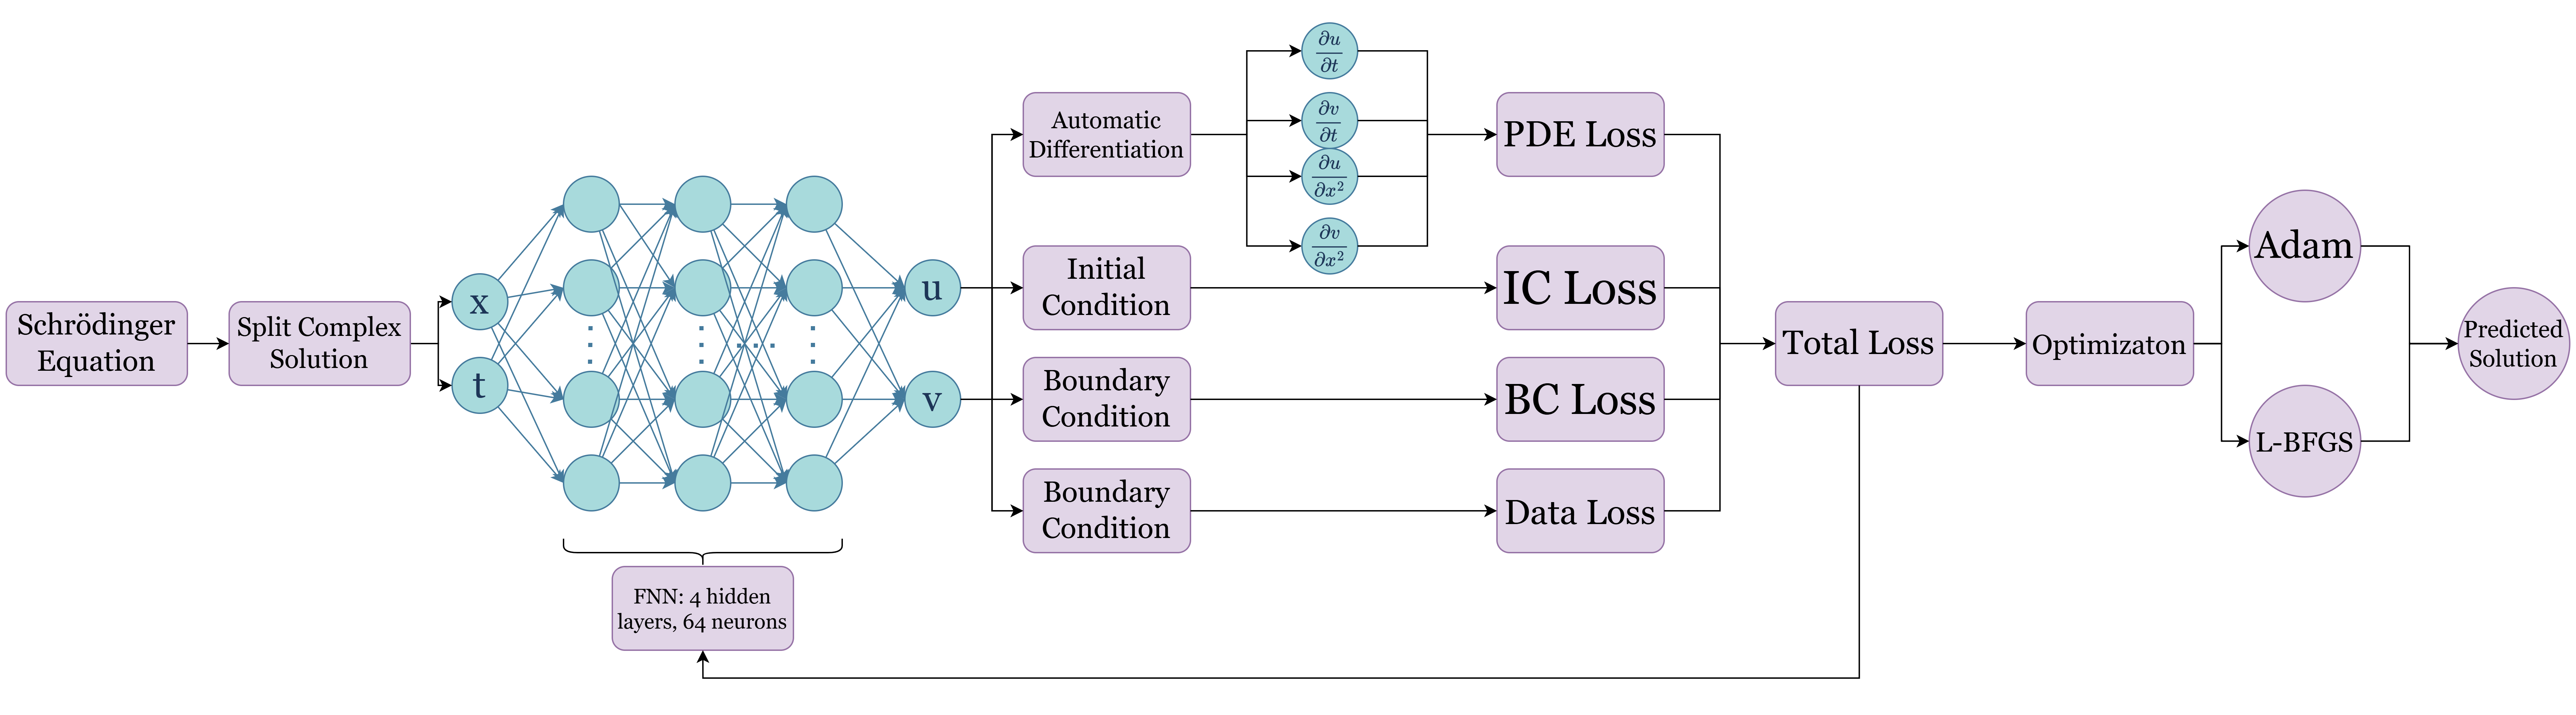
\includegraphics[width=1\textwidth]{SCH_diagram.png}
    \caption{Diagram of solving Schrodinger with PINN}
    \label{fig:sch1}
\end{figure}








\end{document}



